\documentclass{article}

\documentclass[preview,12pt]{article}
\usepackage{amsmath}
\usepackage{gensymb}
\usepackage{ragged2e}
\usepackage{geometry}
\usepackage{graphicx}
\usepackage{caption}
\usepackage{subcaption}
\usepackage{pdfpages}

\geometry{letterpaper, margin=1in}

\begin{document}

\begin{titlepage}
    \vspace*{\fill}
    \begin{center}
        \LARGE \textit{"Measurement of Turbulent Concentration Field of Acetone-Seeded Air Jet using Laser Induced Fluorescence"}
    \end{center}
    \begin{center}
       \large Josh Coffey
    \end{center}
    \begin{center}
        \large University of Cincinnati
    \end{center}
    \begin{center}
        \large November 2019
    \end{center}
        \vspace*{\fill}
\end{titlepage}

\begin{center}
    \section*{Introduction}
\end{center}
\subsection*{Principle of Laser Induced Fluorescence Measurement of Concentration}
\indent Laser induced fluorescence (LIF) is "the spontaneous emission of radiation resulting from the stimulation of an atomic or molecular system by a laser to energies higher than equilibrium"[1].  In other words, the laser beam will excite an atom or molecule to a higher energy state through absorption and when the atom or molecule returns to a lower energy state, it will emit a photon.  The laser is chosen so that it is resonant with the desired transition.  It is a method of measuring the concentration of a species in an airflow.  Unlike other methods of measurement, such as absorption, LIF is not line of sight and gives a point measurement, rather than an average measurement over the laser's path.  In addition, it has the advantage of being non-intrusive, so the measurement does not change the flow field, and real-time, so the measurement taken reflects what is happening at the moment. One of the main disadvantages of LIF is that it is very sensitive to light, including light that is in the background and is not part of the laser.  This can include light from LIF of other species, scattered light from the surroundings, particle incandescence, and gas breakdown. \newline
\indent In LIF, a laser is directed through an air jet.  A detector is set up so that measurements can be taken in the air jet at the point at which the light that reaches the detector intersects with the laser beam passing through the jet. In other words, the fluorescence is measured at 90\degree  from the laser beam.  The measured fluorescence is related to the population of the excited state: the more fluorescence is measured, the higher the population of the excited state.  At thermodynamic equilibrium, the population of the excited state is proportional to the population of the ground state, which gives a value for the population of the desired species.

\subsection*{Measurement Principle for Acetone LIF}
Because the measured fluorescence is proportional to the population of the ground state at thermodynamic equilibrium, the intensity of the fluorescence can be used to find the concentration of the wanted species.  In other words, the concentration of acetone, or whichever tracer is used, is related to the intensity of the laser induced fluorescence of the jet. 
\newline
\indent Quenching is when the fluorescence of a species is reduced, and the main contributor to quenching in LIF is collisional energy losses between particles.  Because the concentration of a species is found because of how much that species fluoresces, anything that reduces that fluorescence will lead to a lower value for species concentration than is actually present.  It is also possible for the opposite to happen: because of a factor outside of the experiment, the fluorescence can increase, thus leading to a higher concentration than is accurate.  \newline
\indent One factor that can affect fluorescence is pressure.  Studies have shown that as pressure increases, so to does the fluorescence, although the effect is reduced as pressure gets higher [2].  In addition, other studies have shown that as pressure increases, quantum efficiency, or the efficiency at which photons are released, increases [3].\newline
\indent Another factor that affects fluorescence is the composition of the gas. The same study that found that the quantum efficiency changes with pressure found that the species that comprises the buffer gas can also change the quantum efficiency [3].  They found that when the buffer gas is air, the quantum efficiency of the acetone decreases, while for nitrogen, methane, and helium the quantum efficiency is not affected.  Another study found that oxygen as the buffer gas increases quenching [5].  Another way that composition changes the fluorescence is in the tracer itself.  While acetone is the most commonly used tracer, it is not the only possibility and each tracer will have different properties [2].  This will have a large impact, on everything from the amount of quenching that occurs to the wavelength of the produced photon. \newline
\indent Temperature can also impact the resulting fluorescence.  One study found that as temperature increases, so to does the wavelength of acetone emissions, and that as temperature increases, the fluorescence of several wavelengths tended to decrease [4].


\newpage
\begin{center}
    \section*{Experimental Setup and Procedure}
\end{center}

\begin{figure}[h]
    \centering
    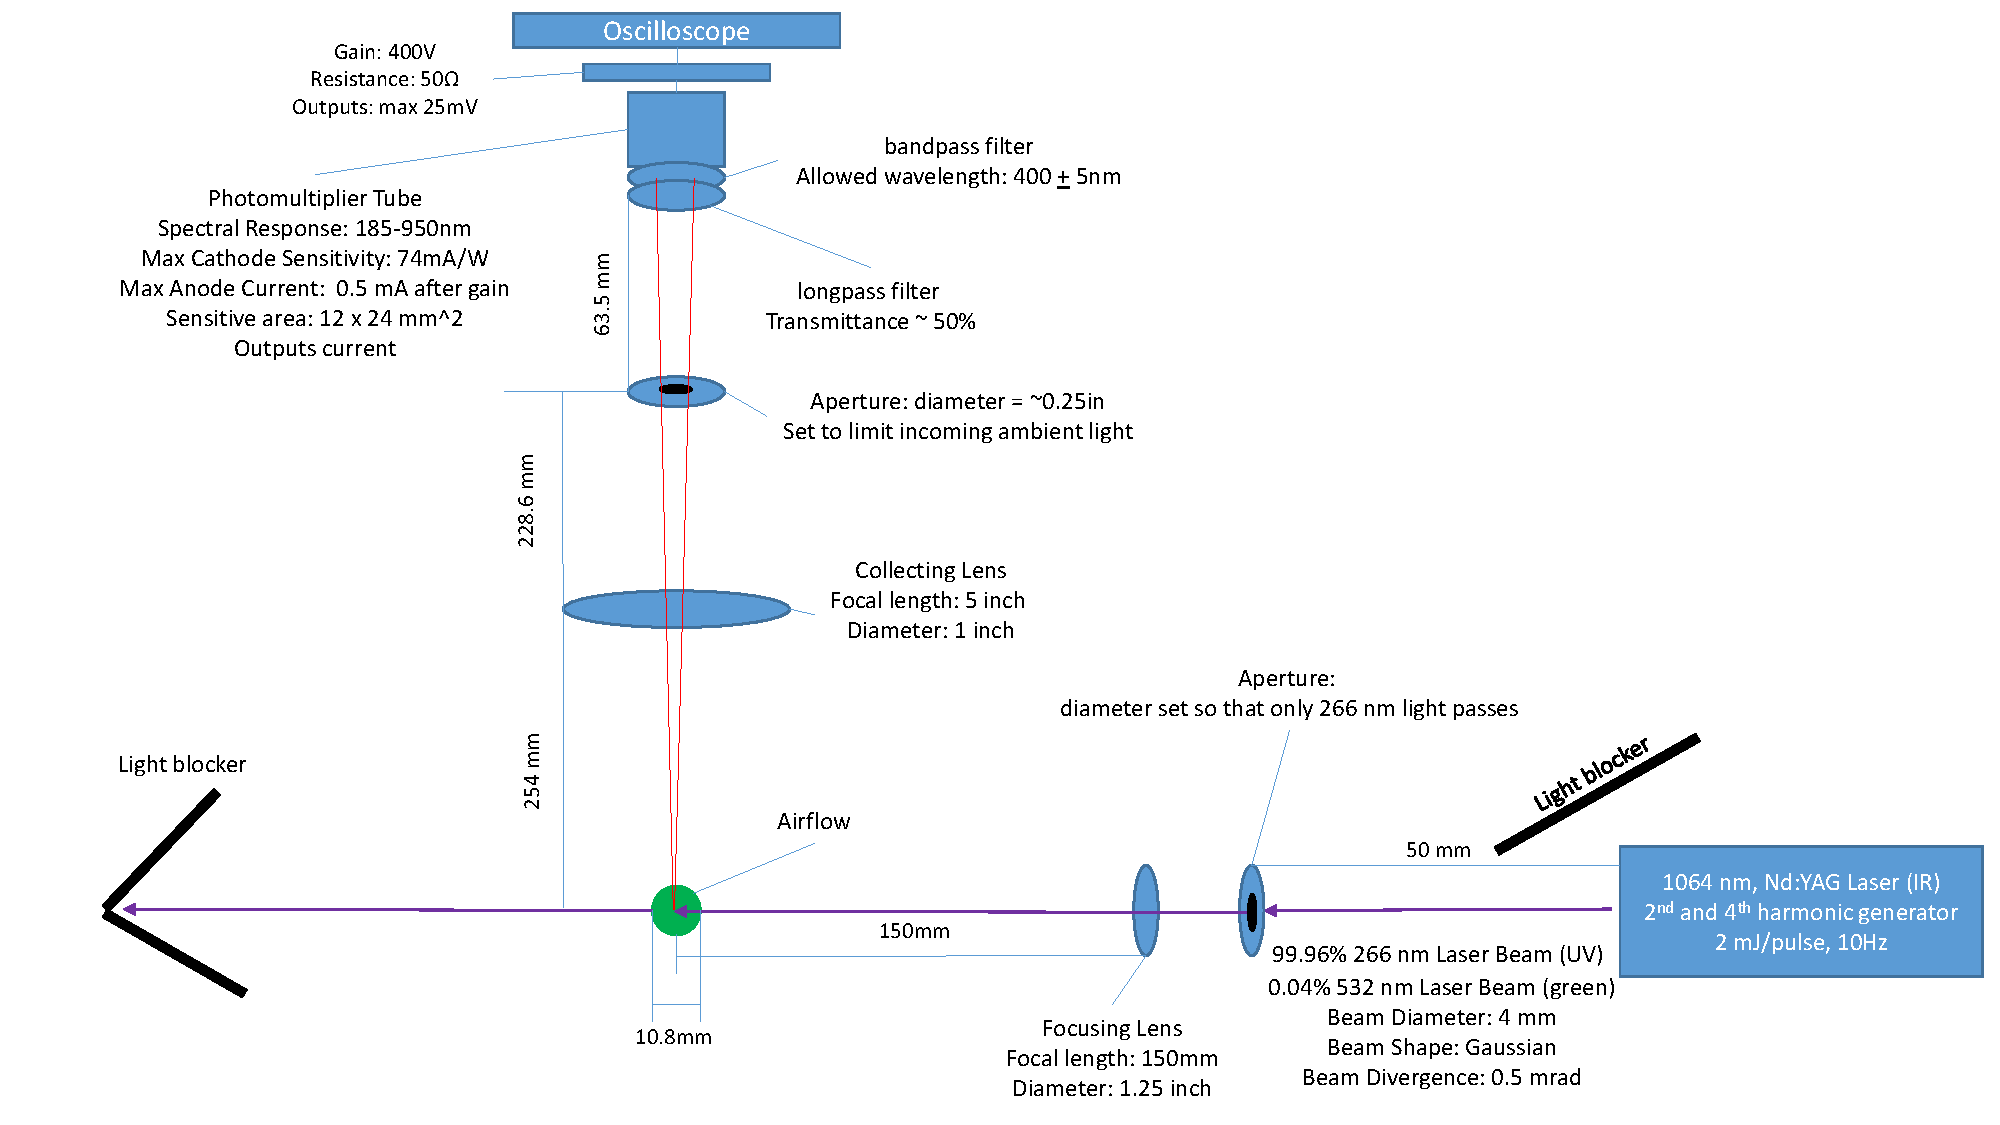
\includegraphics[width=\linewidth]{Lab2Diagram.pdf}
    \caption*{{\footnotesize Figure 1: LIF Lab Setup}}
\end{figure}

This experiment was set up as shown in Figure 1.  The ND:YAG laser produced a beam with a wavelength of 1064 nanometers.  After the second and fourth harmonic generators, there will be three beams of wavelengths 1064 nanometers, 532 nanometers, and 266 nanometers.  As the beam leaves the laser body, the beam makeup will be as shown in figure 1.  The light blocker next to the laser body is meant to block 532 nanometer light from reaching the detector.  The laser beam then passed through an aperture whose diameter was set to prevent any 532 nanometer light from passing through.  This was accomplished by placing a piece of paper on the other side of the aperture.  The 532 nanometer light looked green on the light and the 266 nanometer light looked blue.  The blue light formed a small circle in the center of a larger green circle, so the aperture was slowly closed until only the blue light could be seen.  Next the beam passed through a focusing lens with a focal length of 150 millimeters.  It should be noted that this focal length value was calculated using a 550 nanometer light source which means that the focal length of the lens will be shorter for a light of 266 nanometers.  The laser then passed through the jet of acetone-seeded air, which led to LIF of the acetone.  After the laser passed through the jet, it was directed into a light blocker to end the laser beam.  \newline
\indent The point at which the LIF of the acetone occurred was detected using a photo multiplier tube.  Using a collecting lens and an aperture of approximately one-fourth of an inch, the the fluorescence from the LIF was read by the detector and converted to current.  This current was directed over a resistor of fifty ohms, which, using ohm's law, gave a voltage after a gain of 420 Volts was added of twenty-five millivolts maximum which was able to be read and displayed by an oscilloscope. The values given by the oscilloscope were the magnified voltage values.\newline
\indent To collect data, two values were read from the oscilloscope at different points in the jet.  The first value to be read was the integral of the curve that was displayed on the oscilloscope.  The second value to be read was the average value read on the oscilloscope.  Both of these readings were in voltage. A reading was taken to get the background noise at the first point.\newline
\indent The flow through the jet was made of O2 and acetone seeded N2.  At a Reynolds number of 7500, the velocity of the jet was calculated to be 10.53 m/s which gave a mass flow of 0.00104 kg/s.  The N2 acted as a buffer gas and surrounded the that came from the center of the jet.  Using the control panel in the lab, the mass flow of the air was calculated to be 1.867 SCFM and the mass flow of the N2 was calculated to be 0.346 SCFM.  \newline
\indent Once everything was set up, the jet was moved along a traverse so that it was out of the path of the laser.  Then, the jet was moved one turn so that it moved closer to the laser.  On this traverse, one turn moved the jet 1/20th of an inch.  After each turn, the integration and average voltage at that point was recorded off of the oscilloscope. After approximately 10 turns, another reading of the background was taken with the airflow turned off.  This process was repeated until both data points were maximized, which represented the center of the jet.  After that, five extra data points were taken.
\newline
\begin{center}
    \section*{Results and Discussion}
\end{center}
\indent Figures 2 and 3 (Appendix) represent the the integral of the pulse shown on the oscilloscope and the average reading of the pulse read by the oscilloscope respectively.  These values are directly related to the amount of light that enters the photo multiplier tube in the detector and thus are indicative of the intensity of the LIF emitted by the acetone in the jet. Note that in figure 2 the last point is an increase from the penultimate one, which is likely due to outside light interference, a major source of error in LIF measurements. \newline
\indent The data used in figures 2 and 3 was calculated using the equation:
$$|\textrm{signal read - noise}|$$
where signal read was the value calculated from the oscilloscope at each turn and noise is the value that is shown on the oscilloscope when the experiment is not being run.  The absolute value ensured a positive value for voltage. The radial distance was calculated using the relation:
$$x=\frac{1}{20}(\# turns)$$
and assumes that the beginning position of the traverse is 0.  This gives a value in units of inches. \newline
\indent It can be observed from figures 2 and 3 that the radius of the jet is approximately 1.2 inches minus 0.6 inches or 0.6 inches.  By looking at the raw data and counting the number of turns from beginning of the jet to the center of the jet, the radius can be calculated to be 0.65 inches.  When this is compared to the value gathered through absorption spectroscopy (1.58 cm = 0.62 in), it can be seen that these values are very similar. \newline
\indent In order to measure the absolute acetone concentration, the quantum efficiency would first need to be known.  This would allow you to account for the LIF that is prevented through quenching, and would give the ideal value of LIF of the acetone.  Then, assuming the setup was perfectly ideal and that all the necessary information was known, i.e. laser wavelength and power, focal lengths of lenses, distances between components, etc., then the  laser intensity being absorbed by the acetone can be related to the LIF that is seen, which can then be related to the absolute concentration of acetone in the jet.  \newline
\indent If it is assumed that losses are negligible for an experiment at low pressure and temperature, like the conditions of this lab, then the concentration of acetone can be found.  The total number of moles can be calculated using the ideal gas law where P and T are the ambient pressure and temperature, R is the universal gas constant, and V is found using the diameter $d_s=f\Delta\theta$ and length $L=\frac{\phi_A S}{S"}$.
$$N=\frac{PV}{RT}=\frac{PL\frac{\pi d_s^2}{4}}{RT}=\frac{P\frac{\phi_A S}{S"}\frac{\pi (f\Delta\theta)^2}{4}}{RT}$$
Then, you can find $N_{acetone}$ using the Boltzmann Distribution equation:
$$N_i=\frac{Nge^{(\frac{-E_A}{R_uT})}}{Q}$$
and then the concentration of acetone is:
$$[Acetone]=\frac{N_i}{N}$$
\indent Possible sources of error include: the background interference/noise, assumptions made, and potentially misaligned setups.  The largest source of error would be background interference.  It is known that this is one of the downsides of LIF as a measurement tool, but its effects should be minimized by the background noise measurements taken and used to account for interference in the data.  One way to reduce the interference further is to minimize the amount of ambient light in the area surrounding the experiment, although this may make conducting the experiment difficult.  Another way to solve this issue is to build an enclosure around the system, which would prevent ambient light and make the alignment of the setup much more precise.  However, this may change the air flow behavior, but this may not matter if the only data desired is species concentration.  As mentioned, the alignment is another source of error.  One way to combat this is to have a more precise method of moving the setup so that it is all one system rather than individual parts, but this would reduce the flexibility of the experiment somewhat.  Lastly, several assumptions were made for this experiment which may introduce error to the end result.  One is that all the parts of the experiment are perfectly identical to their rated specifications.  For example, it is assumed that the lenses focal lengths are exact, but this can be somewhat by flaws in the lens.  Another assumption is that the turn wheel on the traverse was turned exactly one full revolution each time, which is unlikely due to simple human error.  Some of these could be avoided through a more rigorous, but time consuming, process, while others are necessary.





\newpage
\begin{center}
    \subsection*{References}
\end{center}
$$$$
\newline
\textbf{1)} Lee, \textit{"Chapter 4: Laser Induced Fluorescence"}, University of Cincinnati Class Notes, Fall 2019 \newline
\textbf{2)}  A. Lozano, B. Yip, and R. K. Hanson, “Acetone: a tracer for concentration measurements in gaseous flows by planar laserinduced fluorescence,” Exp. Fluids 13, 369–376 (1992) \newline
\textbf{3)}  Lucinda S. Yuen, James E. Peters, and Robert P. Lucht, "Pressure dependence of laser-induced fluorescence from acetone," Appl. Opt. 36, 3271-3277 (1997)\newline
\textbf{4)}  Mark C. Thurber, Frédéric Grisch, and Ronald K. Hanson, "Temperature imaging with single-and dual-wavelength acetone planar laser-induced fluorescence," Opt. Lett. 22, 251-253 (1997) \newline
\textbf{5)} M. C. Thurber and R. K. Hanson, "Pressure and composition dependences of acetone laser-induced fluorescence with excitation at 248, 266, and 308 nm," Appl. Phys. B 69, 229-240 (1999) \newline
\textbf{6)} Gabriel Laufer, \textit{Introduction to Optics and Lasers in Engineering}, Cambridge University Press, (1996) \newline

\newpage
\begin{center}
    \section*{Appendix}
\end{center}

\begin{figure}[h]
    \centering
    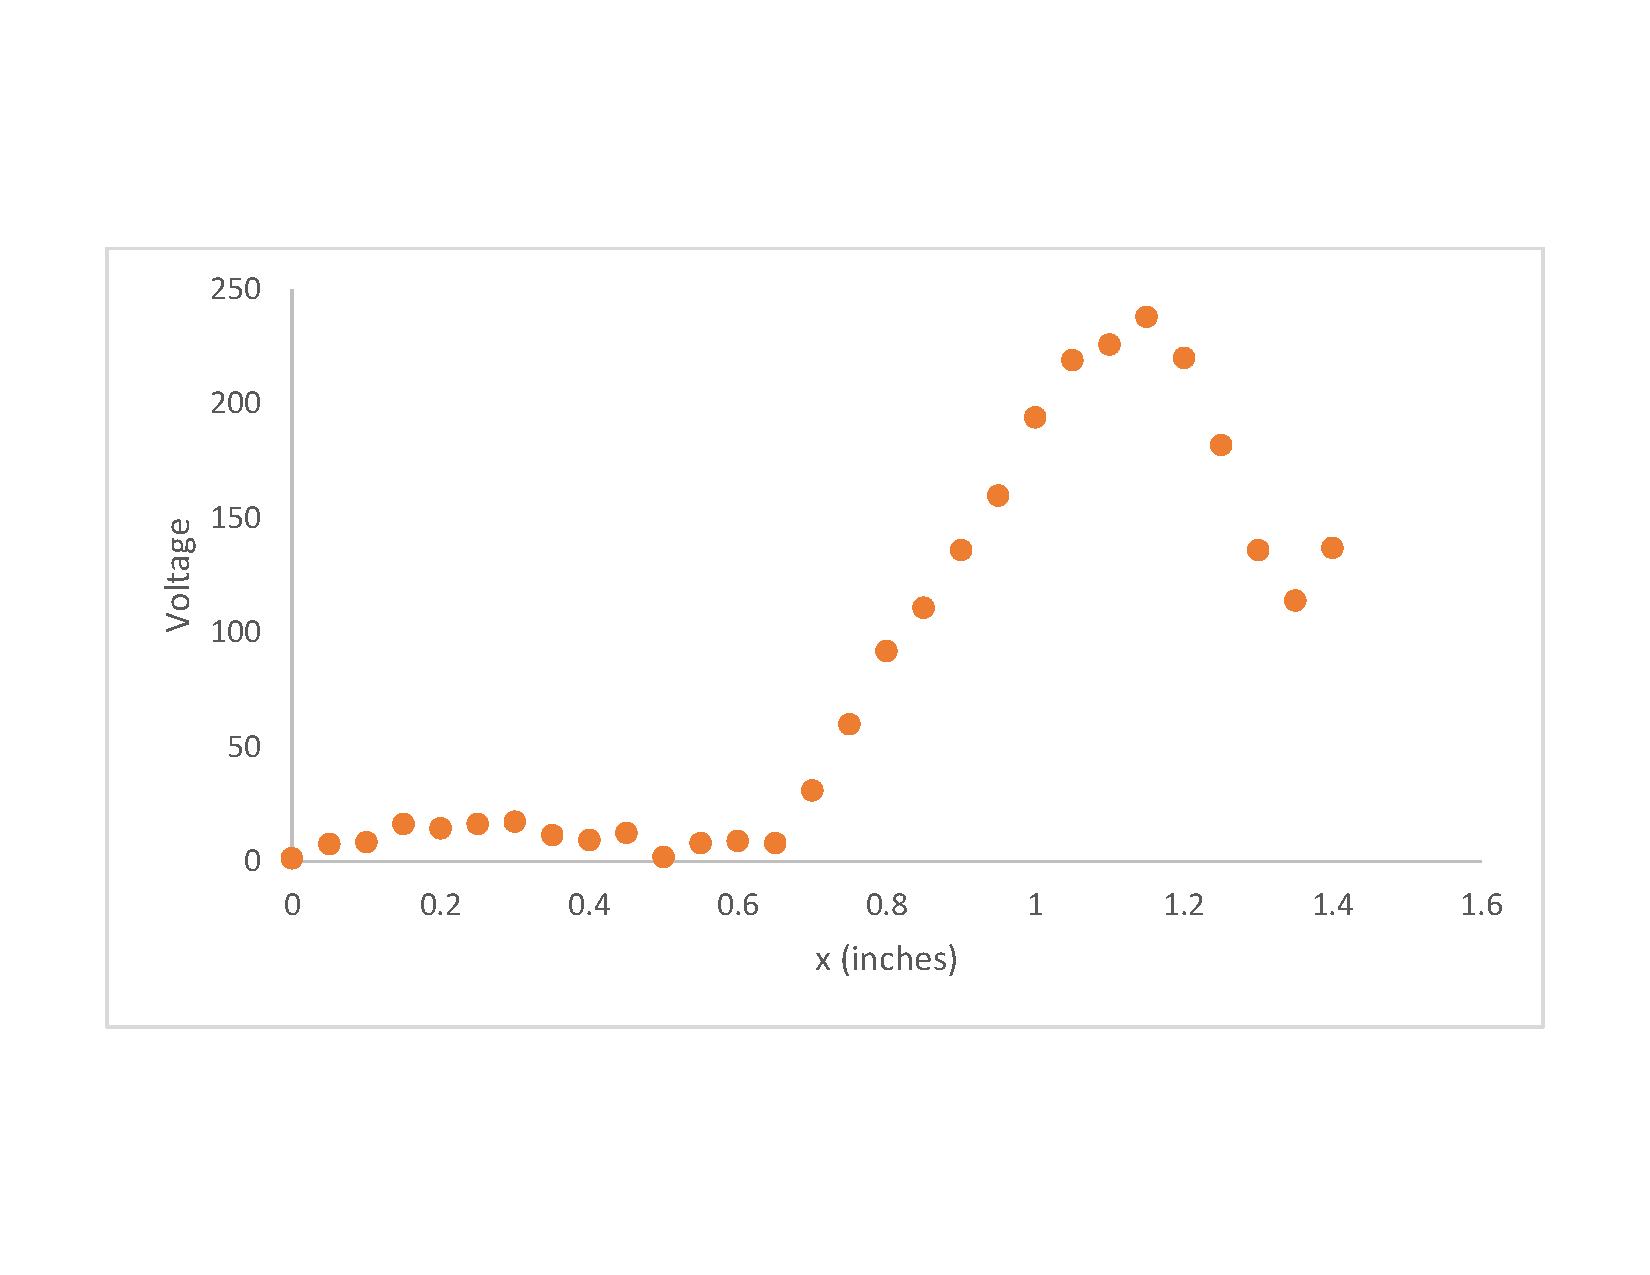
\includegraphics[width=0.6\linewidth]{Lab2Intvsx.pdf}
    \caption*{{\footnotesize Figure 2: Integral of Pulse vs Radial Distance}}
\end{figure}

\begin{figure}[h]
    \centering
    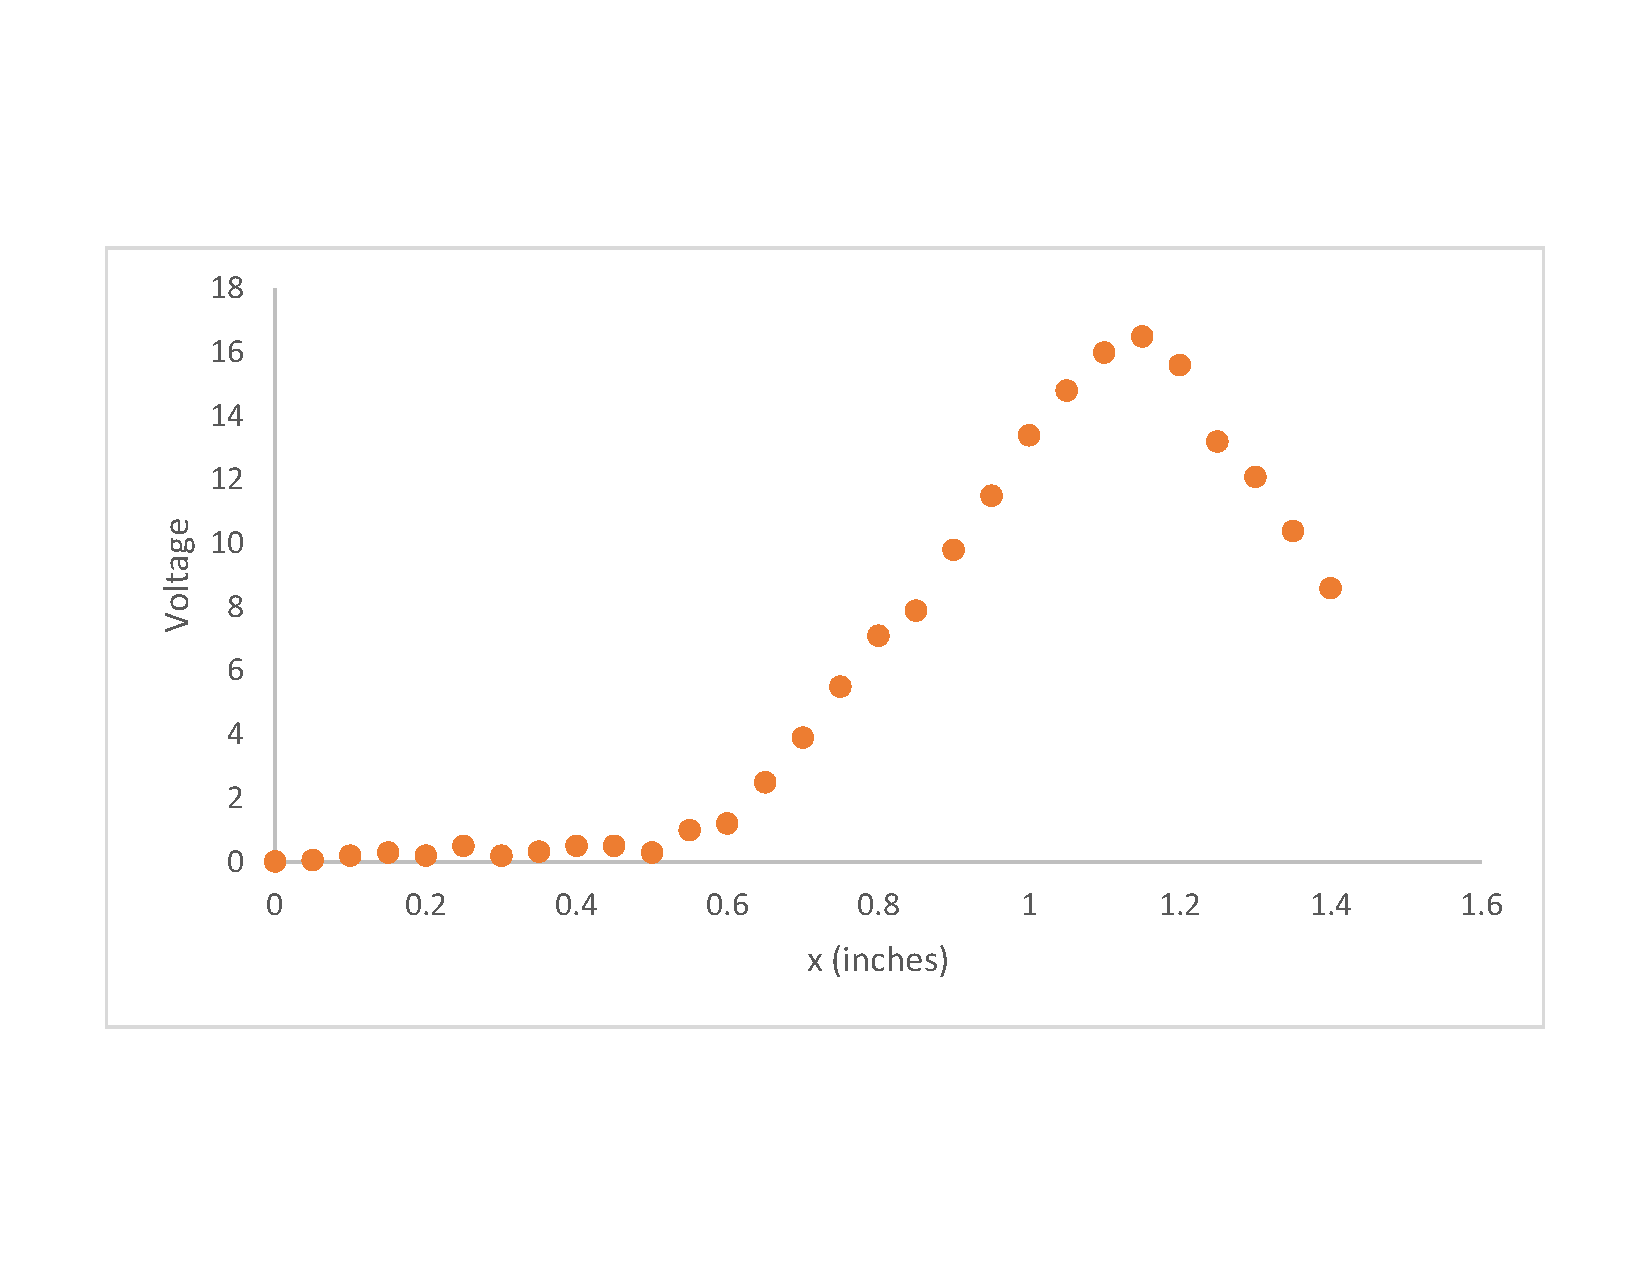
\includegraphics[width=0.6\linewidth]{Lab2avgvsx.pdf}
    \caption*{{\footnotesize Figure 3: Average Voltage of Pulse vs Radial Distance}}
\end{figure}

\end{document}